\chapter{Besoins de l'utilisateur}
\begin{figure}[H]
    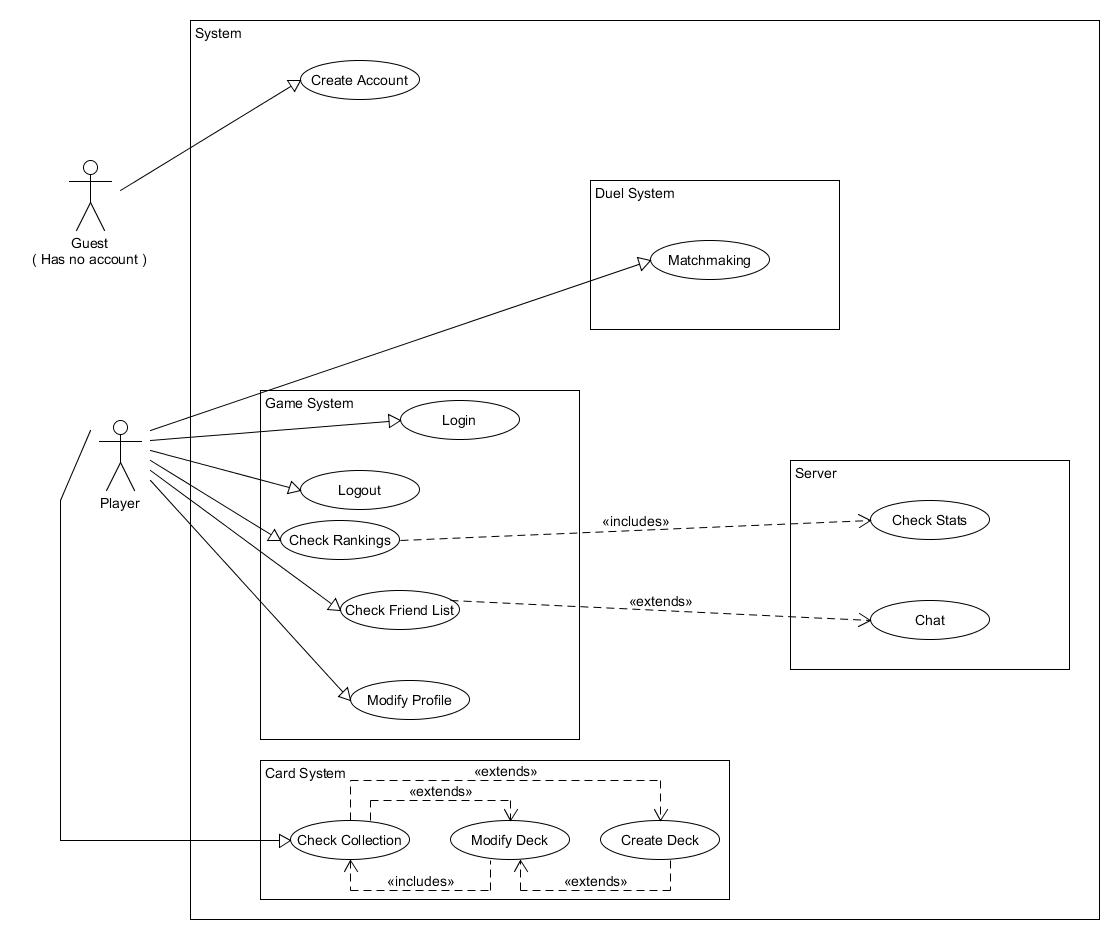
\includegraphics[width=\textwidth]{Images/UseCase.jpg}
    \caption{\label{Use Case} Diagramme Use case du \index{système}système}
\end{figure}

\section{Exigences fonctionnelles}
\subsection{Gestion des utilisateurs}
\begin{itemize}
    \item Cas général  : L'utilisateur doit pouvoir s'inscrire (s'enregistrer) sur le {serveur} avec un nom d'utilisateur unique et un mot de passe.
    \item Pré Condition  : L'utilisateur ne possède pas déjà un \index{account}account.
    \item Post Condition : L'utilisateur aura fait une demande d'inscription.
    \item Cas Exceptionnel : L'inscription échouera et l'utilisateur sera invité à recommencer si le nom de l'\index{account}account est déjà enregistré sur le {serveur}.
\end{itemize}

\subsection{Connexion}

\begin{itemize}
    \item Cas général : L'utilisateur doit pouvoir se connecter auprès du {serveur} avec son identifiant et son mot de passe.
    \item Pré Condition  : L'utilisateur ne s'est pas déjà connecté.
    \item Post Condition : L'utilisateur aura fait une demande de connexion.
    \item Cas Exceptionnel : L'authentification échouera et l'utilisateur sera invité à recommencer si le mot de passe et le pseudonyme ne correspondent pas ou que celui-ci n'est pas reconnu sur le serveur.
\end{itemize}

\subsection{Jouer un tour}
\begin{itemize}
    \item Cas général : L'utilisateur doit pouvoir jouer un tour lors d'un duel\index{duel}, c'est à dire placer ses cartes et/ou effectuer des actions.
    \item Pré Condition  : L'utilisateur doit être dans un duel\index{duel}.
    \item Post Condition : L'utilisateur aura joué ses cartes et actions.
    \item Cas Exceptionnel : Si la connexion est perdu par un des utilisateurs, celui-ci est déclaré comme perdant.
\end{itemize}

\subsection{Déclarer forfait\index{forfait}}
\begin{itemize}
    \item Cas général : L'utilisateur peut déclarer forfait durant un duel\index{duel}.
    \item Pré Condition  : L'utilisateur doit être dans un duel\index{duel}.
    \item Post Condition : L'utilisateur sera déclaré comme perdant.
\end{itemize}

\subsection{Créer un deck}
\begin{itemize}
    \item Cas général : Création d'un nouveau \index{deck}deck via sa \index{collection}collection.
    \item Pré Condition  : L'utilisateur est connecté au serveur et est dans le menu adéquat.
    \item Post Condition : Le deck\index{deck} contient 20 cartes et respecte les conditions d'un deck\index{deck}.
\end{itemize}

\subsection{Matchmaking}
\begin{itemize}
    \item Cas général : L'utilisateur peut initialiser une recherche avec le \index{Matchmaking}.
    \item Pré Condition  : L'utilisateur ainsi que son adversaire sont connectés et ne sont pas dans un \index{duel}.
    \item Post Condition : L'adversaire est connecté aussi en \index{Matchmaking}.
\end{itemize}

\section{Exigences non fonctionnelles}

\subsection{Règles du jeu}
\begin{itemize}[labelindent=16pt]
    \item Il existe deux types de cartes:
        \begin{itemize}[label=\textbullet]
            \item Les spell\index{spell}s sont des cartes ayant un coût en énergie et un effet spécial. Leurs effets varient en fonction de la carte et sont les suivants :
            \begin{itemize}[label=\textasteriskcentered]
                \item Infliger des dégâts 
                \item Soigner une ou plusieurs cibles
                \item Faire apparaître une minion aléatoire
                \item ...
            \end{itemize}
            \item Les minions sont des cartes ayant un coût en énergie, une valeur d'attaque et un montant de points de vie, également appelé Hp. Elles peuvent éventuellement avoir des effets spéciaux tels que:
                \begin{itemize}[label=\textasteriskcentered]
                \item Faire piocher une carte
                \item Augmenter les statistiques d'une autre créature
                \item Invoquer un autre minion
                \item ...
                \end{itemize}
        \end{itemize}
    \item Un deck\index{deck} contient exactement 20 cartes. Les doublons sont acceptés mais le joueur ne peut avoir plus de 2 fois la même carte dans un deck\index{deck}.
    \item Les points d'énergie peuvent être cumulés. Chaque player commence la partie avec 0 point d'énergie. Au début d'un tour, un player voit ses points d'énergie reinitialisés à un. Chaque player peut cumuler jusqu'à 10 points.
    \item A chaque début de tour, le player pioche une carte. Si il en possède déjà 10 en main, cette carte est detruite.
    \item Les players commencent la partie avec 5 cartes en main.
    \item Un \index{système}système va décider aléatoirement quel player à la main au premier tour.
    \item Pseudo code d'un début de tour :
    \begin{itemize}[label=\textasteriskcentered]
        \item $maxPossibleEnergy$++ \textbf{if} $maxPossibleenergy < 10$ \textbf{else} do nothing
        \item $currentPlayer.drawCard()$ \textbf{if} $currentPlayer.handSize < 10$ \textbf{else} $discardCardToDraw()$
        \item $currentPlayer.currentEnergy = currentPlayer.maxPossibleEnergy$
    \end{itemize}
    
\end{itemize}

\subsection{Choix Personnel}
{
\noindent Afin de rendre le gameplay plus intéressant, l'équipe a décidée d'instaurer un \index{système}système de \emph{style}. Un style défini un gameplay, il existe dans l'univers du Wizard Poker plusieurs d'entre eux. Les différents styles auront leurs propres cartes et les decks\index{deck} partageront tous  un ensemble de cartes neutres en plus du style choisi.\\
Le player aura la possibilité de choisir le gameplay qu'il souhaite. L'équilibre entre les cartes appartenant aux styles et les cartes communes sera administré par les soins de l'équipe. Voici deux exemples de styles ainsi que des prototypes de cartes.
}
\subsubsection{Style SinuMonstra}
{
\noindent Ce style se base sur le populaire jeu Pokémon. Les minions de cette classe ont une spécialité. Elles peuvent évolué. Cette évolution rend la carte plus forte en augmentant ses Hps. Les cartes de ce style sont principalement des minions. Mais les quelques spell\index{spell}s ne seront pas des moindres.
\begin{multicols} {3}
\begin{tikzpicture}
% Card
\fill[red!20] (0,0) rectangle (3,5);
% Name
\draw (1.5,4.5) node {Ignicus};
% Mana
\draw (3,5) node[style={rectangle, fill=blue!40, very thick, minimum size=5mm}] {1};
% Health
\draw (3,0) node[style={rectangle, fill=red!40, very thick, minimum size=5mm}] {2};
% Attack
\draw (0,0) node[style={rectangle, fill=gray!40, very thick, minimum size=5mm}] {1};
% Artwork
\draw (1.5,3) node {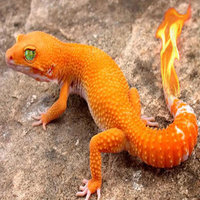
\includegraphics[width=2cm, height=2cm]{Images/Artwork/ignicus.jpg}};
% Description
\draw (1.5,1) node[align=center,text width=3cm] {\tiny{The flame on his tail is as much a live-saver as a burden. A de-ignited Ignicus will slowly die.\par}};
\end{tikzpicture}
\vfill
\columnbreak
\begin{tikzpicture}
% Card
\fill[red!20] (0,0) rectangle (3,5);
% Name
\draw (1.5,4.5) node {Turqua};
% Mana
\draw (3,5) node[style={rectangle, fill=blue!40, very thick, minimum size=5mm}] {1};
% Health
\draw (3,0) node[style={rectangle, fill=red!40, very thick, minimum size=5mm}] {2};
% Attack
\draw (0,0) node[style={rectangle, fill=gray!40, very thick, minimum size=5mm}] {1};
% Artwork
\draw (1.5,3) node {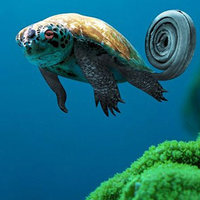
\includegraphics[width=2cm, height=2cm]{Images/Artwork/turqua.jpg}};
% Description
\draw (1.5,1) node[align=center,text width=3cm] {\tiny{It dreams of a day when it can finally kill the sharks that preyed on his siblings.\par}};
\end{tikzpicture}
\vfill
\columnbreak
\begin{tikzpicture}
% Card
\fill[red!20] (0,0) rectangle (3,5);
% Name
\draw (1.5,4.5) node {Bulstrum};
% Mana
\draw (3,5) node[style={rectangle, fill=blue!40, very thick, minimum size=5mm}] {1};
% Health
\draw (3,0) node[style={rectangle, fill=red!40, very thick, minimum size=5mm}] {2};
% Attack
\draw (0,0) node[style={rectangle, fill=gray!40, very thick, minimum size=5mm}] {1};
% Artwork
\draw (1.5,3) node {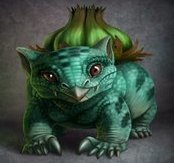
\includegraphics[width=2cm, height=2cm]{Images/Artwork/bulstrum.jpg}};
% Description
\draw (1.5,1) node[align=center,text width=3cm] {\tiny{Its brain is the size of a Stegosaurus', it can't be said it is very smart.\par}};
\end{tikzpicture}
\end{multicols}
}
\subsubsection{Style ULB}
{
\noindent Ce style se base sur l'Université Libre de Bruxelles. Elle comporte des minions surpuissants appelés \emph{Professeur} qui sont très efficaces contre des minions de type \emph{Étudiant}. Ces cartes de type Professeur pourront attaquer un type \emph{Étudiant} ou au contraire augmenter ses Hps.
\begin{multicols} {3}
\begin{tikzpicture}
% Card
\fill[blue!20] (0,0) rectangle (3,5);
% Name
\draw (1.5,4.5) node {Msr. Roggeman};
% Mana
\draw (3,5) node[style={rectangle, fill=blue!40, very thick, minimum size=5mm}] {10};
% Health
\draw (3,0) node[style={rectangle, fill=red!40, very thick, minimum size=5mm}] {8};
% Attack
\draw (0,0) node[style={rectangle, fill=gray!40, very thick, minimum size=5mm}] {8};
% Artwork
\draw (1.5,3) node {
\includegraphics[width=2cm, height=2cm]{Images/Artwork/yves.jpg}};
% Description
\draw (1.5,1) node[align=center,text width=3cm] {\tiny{\textbf{Effect:} Whenever a student is summonded set their attack to 0.\\He wll not be taken down by them.\par}};
\end{tikzpicture}
\vfill
\columnbreak
\begin{tikzpicture}
% Card
\fill[blue!20] (0,0) rectangle (3,5);
% Name
\draw (1.5,4.5) node {Keno Merckx};
% Mana
\draw (3,5) node[style={rectangle, fill=blue!40, very thick, minimum size=5mm}] {7};
% Health
\draw (3,0) node[style={rectangle, fill=red!40, very thick, minimum size=5mm}] {6};
% Attack
\draw (0,0) node[style={rectangle, fill=gray!40, very thick, minimum size=5mm}] {5};
% Artwork
\draw (1.5,3) node {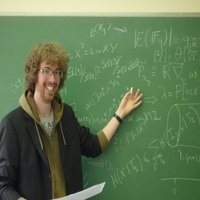
\includegraphics[width=2cm, height=2cm]{Images/Artwork/keno.jpg}};
% Description
\draw (1.5,1) node[align=center,text width=3cm] {\tiny{\textbf{Effect:} Give ALL students +2/+2.\\He wants them to be succesfull.\par}};
\end{tikzpicture}
\vfill
\columnbreak
\begin{tikzpicture}
% Card
\fill[blue!20] (0,0) rectangle (3,5);
% Name
\draw (1.5,4.5) node {TD a la Jefke};
% Mana
\draw (3,5) node[style={rectangle, fill=blue!40, very thick, minimum size=5mm}] {4};
% Artwork
\draw (1.5,3) node {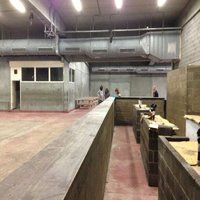
\includegraphics[width=2cm, height=2cm]{Images/Artwork/jefke.jpg}};
% Description
\draw (1.5,1) node[align=center,text width=3cm] {\tiny{\textbf{SPELL}\\ All students become inmune and have +5 attack this turn\par}};
\end{tikzpicture}
\end{multicols}
}
\section{Exigences du domaine}
{
\noindent Le domaine de ce projet étant le domaine du jeu-video, il n'y a pas de contraintes communes et absolues à tous les jeux-vidéos. Ceci nous laisse donc une grande liberté de prise de décision sur les contraintes du domaine de Wizard Poker.
}